Prévio ao processo de calibração foi realizado um processo de Pré-processamento dos dados para reduzir ruído e quantidade de \textit{outliers}. Para isso os dados foram etiquetados seguindo alguns pontos dos procedimentos descritos por \textit{AQMesh}, Ottosen e Kumar \cite{Ottosen2019OutlierMeasurements} e o Guia para monitoramento da qualidade do ar o IMA \cite*{INSTITUTODEENERGIAEMEIOAMBIENTE2019QualidadeAr}. O pré-processamento foi realizado utilizando a linguagem de programação Python e \textit{Jupyter Notebooks}. A continuação detalham-se as etiquetas utilizadas, entre parênteses é colocado o nome da etiqueta utilizada dentro do código. Os Anexos XXX a XXX contêm o código desenvolvido em \textit{Jupyter Notebooks} para o processo de filtragem dos dados dos sensores.

\begin{itemize}
    \item Dados faltantes (\textit{MISSING}): Esta etiqueta representa amostras faltantes na amostragem dos dados.
    \item Estabilização (\textit{STABILIZ}): A estabilização é um período em que um sensor fornece dados não confiáveis por não estar em estado de equilíbrio. Uma vez que o sensor se estabilizar em seu ambiente após ter sido movido recentemente ou após ter sido instalado pela primeira vez, ele fornecerá dados utilizáveis. Este processo leva 2 dias para ser concluído para sensores eletroquímicos, não sendo necessário para o sensor de material particulado modelo OPC de Alphasense (Manual de procedimento de operação padrão AQMesh). Neste trabalho foi utilizado um período de 7 dias para garantir uma maior estabilidade do sensor.
    \item Dados acima do Limite Superior (\textit{GTUL}): Essa etiqueta está relacionada a valores que ultrapassam o limite superior do sensor. As especificações do fabricante ou valores conhecidos do poluente podem ser utilizados para definir esse limite. Por exemplo, o sensor Alphasense CO-B4 tem um limite de 1.000 ppm, equivalente a 1.000.000 ppb. Os valores que ultrapassaram esses limites para cada sensor foram removidos por serem indícios de alguma falha ou mal funcionamento do sistema de medição.
    \item Dados abaixo do Limite Inferior (\textit{LTLL}): Esta etiqueta sugere valores que estão abaixo da resolução do sensor e pode estar relacionada a possíveis valores negativos. A definição desse limite depende das especificações do sensor utilizado. O sistema de medição desenvolvido identifica valores faltantes ou NaN com o valor -9999.99. Por esse motivo, valores abaixo de -1000 ppb nos dados representam estas amostras depois de passar pelo processo de suavização.
    \item Dados com alteração do valor de linha base (\textit{REBASE}): Nas séries temporais dos sensores foram identificados alterações no valor de linha base das leituras. Observou-se também que nesses intervalos de variação da linha base a distribuição dos dados também estava alterada. Por esse motivo, os dados nesses intervalos foram marcados e removidos.
    \item Dados do quartil 99 \% (\textit{GTQTLE99}): Essa etiqueta está relacionada aos valores que se encontram no quartil 99 \% no histograma dos dados. Valores dentro desse intervalo foram etiquetados para remoção.
    \item Dados do quartil 1 \% (\textit{LTQTLE01}): Essa etiqueta está relacionada aos valores que se encontram no quartil 1 \% no histograma dos dados. Valores dentro desse intervalo foram etiquetados para remoção.
    \item Baixo número de amostras (\textit{LOWSAMPLES}): De acordo com o Guia de Monitoramento da Qualidade do Ar (IMA), pelo menos 3/4 das medições de uma hora devem ser válidas para o cálculo da média horária. No sistema desenvolvido, como o período de amostragem foi de 15 minutos, para uma média horária ser considerada válida, ela deve ser calculada por 3 ou 4 pontos.
    \item Transições abruptas nos dados (\textit{BADSPIKE}): Transições muito abruptas na série de dados também foram identificados. Para isso foram calculadas as derivadas das séries temporais e os valores comparados com o valor máximo das derivadas das séries temporais de referência. Valores de derivadas na série de dados acima desse valor máximo foram identificados como transições muito abruptas e etiquetados para remoção.
    \item Dados inválidos de temperatura \textit{INVALID\_ENV}: Aos dados de temperatura também foram aplicadas as etiquetas descritas anteriormente, com exceção de \textit{STABILIZ} e \textit{BADSPIKE}. Os valores de concentração de gás adquiridos no mesmo instante de algum dado inválido de temperatura foram marcados como \textit{INVALID\_ENV} para remoção.    
\end{itemize}

\subsection{Metodologia de preprocessamento das séries temporais}

Utilizando as etiquetas mencionadas anteriormente, foi aplicada uma metodologia de pré-processamento para remoção de ruído e outliers, conforme descrito a continuação.

\begin{enumerate}
    \item Suavização das curvas de dados com uma janela temporal de 1 hora: Primeiramente foi realizada a suavização das séries originais buscando reduzir o impacto de flutuações de curto prazo e realçar padrões de longo prazo, dado que os dados de referência encontram-se em períodos horários.
    \item Remoção do Período de Estabilização: Os primeiros 7 dias da série temporal foram desconsiderados. Essa decisão fundamenta-se na consideração de que nesse período inicial após a instalação o sensor encontra-se num estado de estabilização propenso a flutuações e ajustes. A remoção desses dados iniciais visa mitigar possíveis distorções na análise decorrentes desse período transitório.
    \item Remoção de valores fora de intervalo de medição: Em seguida, foram removidos os valores abaixo da resolução do sensor e acima do valor máximo do sensor. Tal procedimento tem por objetivo eliminar possíveis ruídos, registros muito extremos e falhas no sistema de medição que poderiam comprometer a integridade da série temporal.
    \item Remoção de valores com alterações na linha base: Para a detecção dos pontos em que a linha base das leituras sofreu alterações aplicou-se algoritmo \acrshort{pelt} \cite{Killick2012OptimalCost}. Este método foi aplicado por Ottosen e Kumar \cite{Ottosen2019OutlierMeasurements} para detectar mudanças abruptas na média e/ou na variância das séries temporais de sensores de gases. As leituras que apresentaram alterações na linha base foram desconsiderados já que nesses intervalos a distribuição dos dados também mudava e não apenas a linha base.
    \item Remoção de outliers por quartis: Consistiu na remoção dos quartis 1\% e 99\% dos dados agrupados por hora. Esse processo foi conduzido após a divisão dos dados em 24 grupos, representando cada hora do dia. Os quartis foram calculados individualmente dentro desses grupos, resultando em uma eliminação robusta de extremos estatísticos que poderiam introduzir viés na análise.
    \item Identificação e remoção de picos e outliers na derivada dos dados: Este passo envolveu a identificação e eliminação de picos na primeira derivada dos dados que excediam o valor máximo encontrado na derivada da série de dados de referência. Essa estratégia visa mitigar efeitos de variações abruptas, frequentemente associadas a falhas no sensor ou interferências externas.
    \item Re-amostragem para período de 1 hora: Este passo consistiu na re-amostragem dos dados para um período de 1 hora. Essa prática foi adotada para comparar e calibrar com os dados de referência que estão em períodos de uma hora.
    \item Remoção de médias com amostras insuficientes: Por fim, foram excluídas as médias de cada hora que não atingiram mais de 75\% de amostras válidas, equivalente a pelo menos 3 amostras por hora. Essa medida visa garantir a robustez estatística das médias horárias, excluindo intervalos com dados insuficientes para uma análise significativa.
\end{enumerate}

\subsection{Preprocessamento dos dados de Monóxido de Carbono}

A metodologia de pre-processamento dos dados descrita acima foi aplicada as leituras obtidas pelo sensor de \acrshort{co}. A Figura \ref{fig:data-co-raw} mostra a série temporal do sensor depois de removidos os valores fora de intervalo. Observa-se que a partir do mês de fevereiro ocorreram seguidas alterações de linha base que foram detectadas pelo algoritmo \acrshort{pelt}, conforme ilustrado na Figura \ref{fig:data-rebase-co}. Dado que as mudanças de linha base se mantiveram de forma continuada a partir desse mês, para o restante das análises apenas foram consideradas as leituras anteriores à primeira alteração da linha base do sensor. As Figuras \ref{fig:data-co-preproc-15} e \ref{fig:data-co-preproc-1HR} mostram a série de dados do sensor CO-B4 depois de aplicado o pré-processamento com períodos de 15 minutos e 1 hora respectivamente. 

A Tabela \ref{tab:data-contab-co} mostra a contabilização dos dados para período de 15 minutos e de 1 hora. Observa-se que dos 17647 pontos de dados, que representavam as amostras adquiridas com um período de 15 minutos no intervalo de 20/11/2022 até 23/05/2023, 4270 foram aproveitados como dados válidos, o que representa um 24 \% aproximadamente dos dados originais. Ao re-amostrar esses 4270 pontos em dados horários obtiveram-se 1048 amostras horárias de concentração válidas (aproximadamente 64 \% dos dados) para realizar a calibração.

\begin{figure}[h]
    \centering
    \caption{Série temporal do sensor CO-B4}
    \begin{subfigure}{0.495\textwidth}
        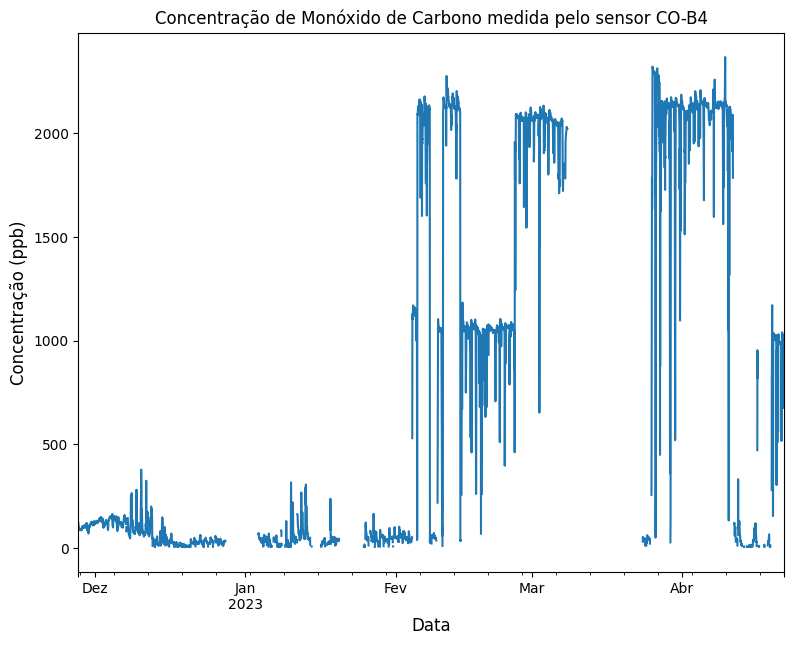
\includegraphics[width=\textwidth]{chapters/3-RESULTADOS CAMPO/Figuras/raw-co-b4.png}
        \caption{Série temporal do sensor depois de remover valores fora de intervalo}
        \label{fig:data-co-raw}
    \end{subfigure}
    \hfill
    \begin{subfigure}{0.495\textwidth}
        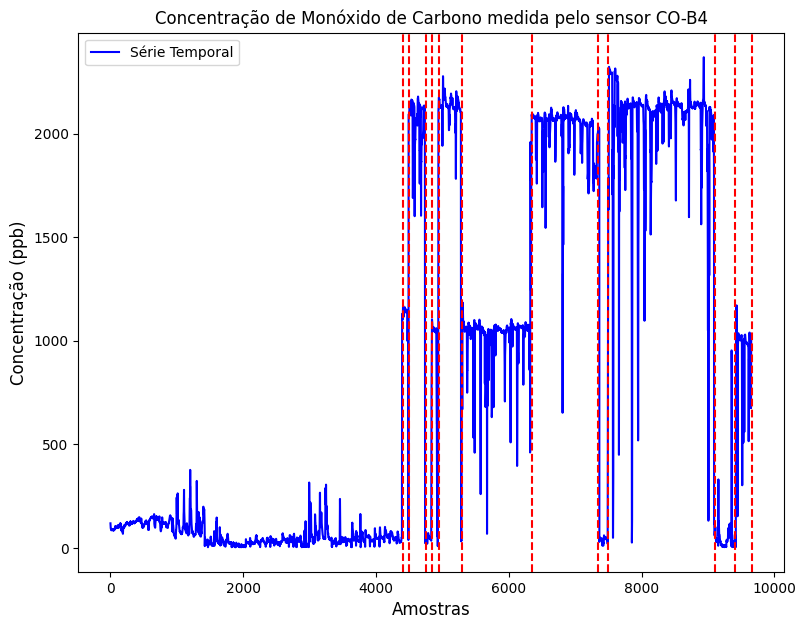
\includegraphics[width=\textwidth]{chapters/3-RESULTADOS CAMPO/Figuras/rebase-co-b4.png}
        \caption{Pontos de alteração da linha base detectados pelo algoritmo \acrshort{pelt}}
        \label{fig:data-rebase-co}
    \end{subfigure}
    \hfill
    \label{fig:data-co-raw-and-pelt}
    \fonte{Desenvolvido pelo autor (2023)}
\end{figure}

\begin{figure}[h]
    \centering
    \caption{Série temporal do sensor CO-B4 pré-processada}
    \begin{subfigure}{0.495\textwidth}
        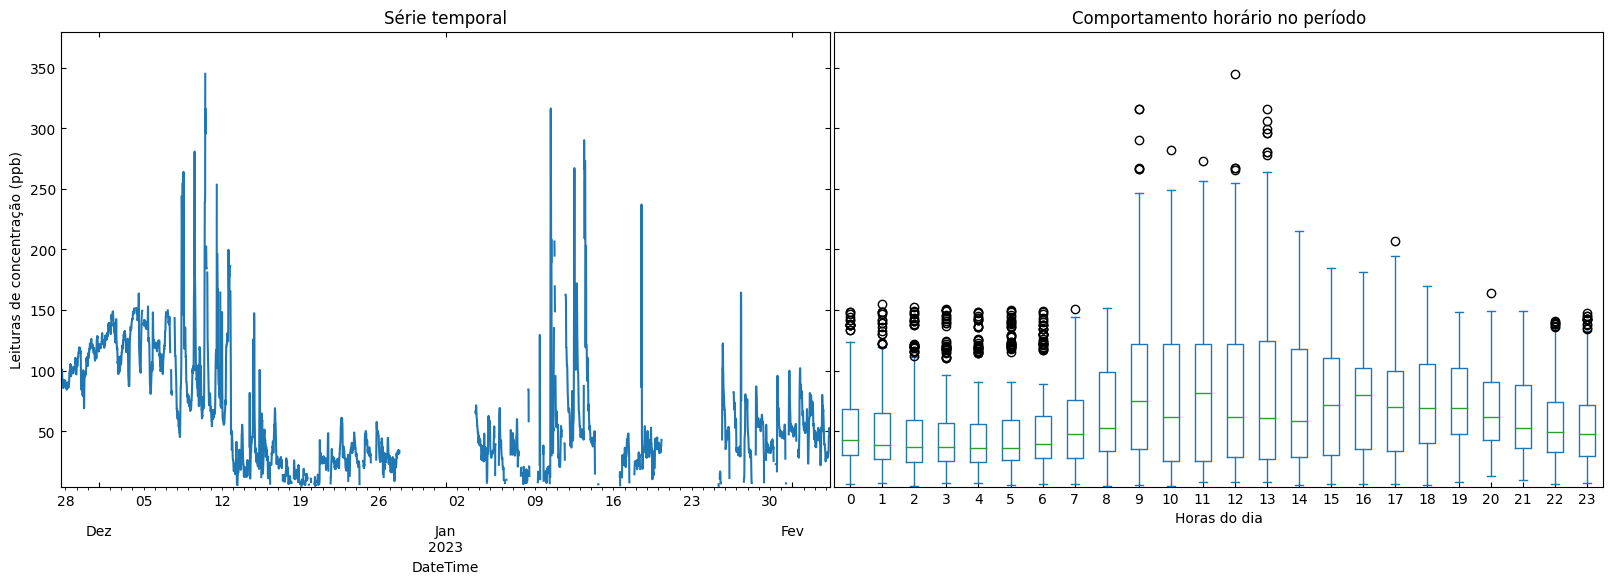
\includegraphics[width=\textwidth]{chapters/3-RESULTADOS CAMPO/Figuras/preproc-co-b4.png}
        \caption{Série temporal do sensor pré-processada (T = 15 mins)}
        \label{fig:data-co-preproc-15}
    \end{subfigure}
    \hfill
    \begin{subfigure}{0.495\textwidth}
        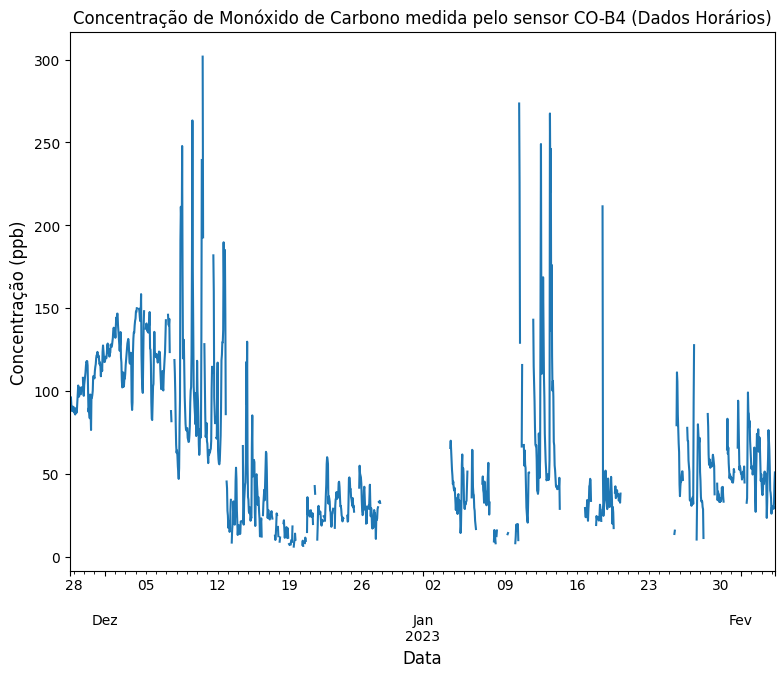
\includegraphics[width=\textwidth]{chapters/3-RESULTADOS CAMPO/Figuras/preproc-1HR-co-b4.png}
        \caption{Série temporal do sensor pré-processada (T = 1 hr)}
        \label{fig:data-co-preproc-1HR}
    \end{subfigure}
    \hfill
    \label{fig:data-co-preproc}
    \fonte{Desenvolvido pelo autor (2023)}
\end{figure}

\begin{table}[t]
    \caption{Contabilização dos dados por etiquetas das leituras do sensor CO-B4}
    \centering
    \begin{tabularx}{0.95\textwidth}[h]{
         >{\raggedright\hsize=.45\hsize\arraybackslash}X
         >{\raggedright\hsize=.20\hsize\arraybackslash}X 
         >{\raggedright\hsize=.5\hsize\arraybackslash}X
         >{\raggedright\hsize=.50\hsize\arraybackslash}X 
         >{\raggedright\hsize=.20\hsize\arraybackslash}X 
         >{\raggedright\hsize=.5\hsize\arraybackslash}X }
        \multicolumn{3}{c}{Série temporal T = 15 mins} & \multicolumn{3}{c}{Série temporal T = 1 hr} \\
        \hline
        Etiquetas & No. amostras & \% amostras & Etiquetas & No. amostras & \% amostras \\ [0.5ex]
        \hline
        \textit{MISSING} & 1194 & 6.77 \% & \textit{LOWSAMPLES} & 603 & 36.52 \% \\ [0.5ex]
        
        \textit{LTLL} & 1020 & 5.78 \% & \textit{VALID} & 1048 & 63.48 \% \\ [0.5ex]
        
        \textit{GTUL} & 0 & 0.0 \% & & & \\ [0.5ex]
        
        \textit{STABILIZING} & 649 & 3.68 \% & & & \\ [0.5ex]
        
        \textit{BADSPIKE} & 4351 & 24.66 \% & & & \\ [0.5ex]
        
        \textit{LTQTLE01} & 63 & 0.36 \% & & & \\ [0.5ex]
        
        \textit{GTQTLE99} & 58 & 0.34 \% & & & \\ [0.5ex]
        
        \textit{REBASE} & 6042 & 34.24 \% & & & \\ [0.5ex]
        
        \textit{VALID} & 4270 & 24.20 \% & & & \\ [0.5ex]
        \hline
        TOTAL & 17647 & & TOTAL & 1651 & \\
    \end{tabularx}
    \label{tab:data-contab-co}
    \fonte{Desenvolvido pelo autor}
\end{table}

\subsubsection{Dependência com a temperatura}

Investigou-se a existência de correlação entre as leituras do sensor de \textit{co} e as variações de temperatura medida no interior da câmara de medição. Para tal, foram empregados os testes estatísticos de correlação de Spearman e Kendall, por serem métodos não paramétricos que exploram a relação monotônica entre variáveis. Os resultados desses testes revelaram coeficientes de correlação significativos. O coeficiente de Spearman calculado foi de 0.521, com um valor de p inferior a 0.05, indicando uma correlação estatisticamente significativa entre as leituras do sensor e a temperatura. De maneira semelhante, o coeficiente de Kendall foi de 0.379, também com p < 0.05, reforçando a presença de uma associação significativa. Ao avaliar a hipótese nula de ausência de correlação, os resultados forneceram evidências robustas para sua rejeição, sugerindo que há uma correlação entre as leituras do sensor de \acrshort{co} e as variações de temperatura. A Figura X mostra um gráfico de dispersão entre os dados do sensor e a temperatura, ilustrando os resultados de correlação obtidos.

\begin{figure}[h]
    \centering
    \caption{Relação entre as leituras do sensor CO-B4 e a temperatura}
    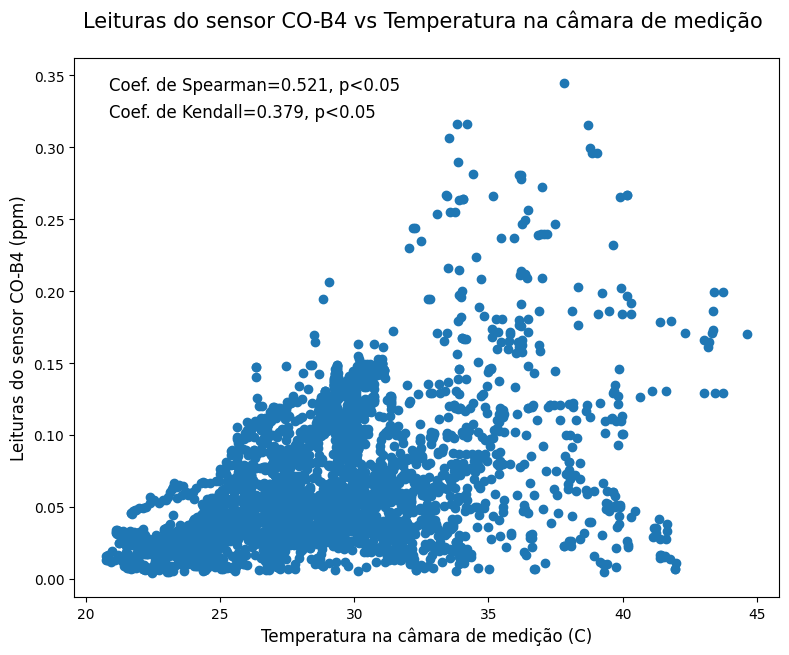
\includegraphics[width=\textwidth]{chapters/3-RESULTADOS CAMPO/Figuras/temperature-co-b4.png}
    \label{fig:data-temp-co-corr}
    \fonte{Desenvolvido pelo autor (2023)}
\end{figure}

\subsection{Preprocessamento dos dados de Dióxido de Nitrogênio}
